% !TeX root = RJwrapper.tex
\title{Kernel Heaping - Kernel Density Estimation from regional aggregates via measurement error model}


\author{by Lorena Gril, Laura Steinkemper, Marcus Groß, and Ulrich Rendtel}

\maketitle

\abstract{%
The phenomenon of ``aggregation'' often occurs in the regional
dissemination of information via choropleth maps. Choropleth maps
represent areas or regions that have been subdivided and color-coded
proportionally to ordinal or scaled quantitative data. By construction
discontinuities at the boundaries of rigid aggregation areas, often of
administrative origin, occur and inadequate choices of reference areas
can lead to errors, misinterpretations and difficulties in the
identification of local clusters. However, these representations do
not reflect the reality. Therefore, a smooth representation of
georeferenced data is a common goal. The use of naive non-parametric
kernel density estimators based on aggregates positioned at the
centroids of the areas result also in an inadequate representation of
reality. Therefore, an iterative method based on the Simulated
Expectation Maximization algorithm was implemented in the
Kernelheaping package. The proposed approach is based on a partly
Bayesian algorithm treating the true unknown geocoordinates as
additional parameters and results in a corrected kernel density
estimate.
}

\section{Introduction}

The data represented by area aggregates do not offer the precise geocoordinates, but they rather refer to areas, usually of varying sizes, such as states, provinces, municipalities, electoral districts, ZIP codes or other statistical spatial references.
These data are mostly displayed by  choropleth maps.
On the one hand, the reason for this type of presentation is that data were not collected at a more granular level. 
For example, election results can only be traced back to the corresponding constituency in order to maintain election secrecy of the voters.
On the other hand, the data with precise geoinformation are often aggregated due to privacy reasons of the participants of a survey or a census survey. Here, data aggregation is a simple strategy of data anonymization.
One drawback of choropleth maps are strong variations  of the distribution density at the borders of the reference areas which make it difficult to identify regional clusters and lead to   misinterpretations of choropleth maps. 
The representation of data as aggregates leads to the fact that this underlies the specific areal map base.
In the so-called support problem, one would like to construct a map based on a different area system which is not hierarchically nested in the original area system.
For example, we want aggregates for administrative districts, but we only have access to aggregates at the ZIP code level. It is by no means obvious how the original total numbers are distributed across the preferred areas.\\

From the statistical point of view, both problems could be addressed with a solid methodological input.
The first step is to search for statistical tools that solve the above problems, given full access to the geocoordinates of each observation.
A good candidate is the two-dimensional kernel density estimate, which provides a smooth regional distribution of the variable of interest without discontinuities. 
Moreover, the kernel density is not linked to a specific reference areas. 
However, to construct a kernel density estimate, we need to know the original geocoordinates.
When using aggregated data by means of a naive kernel density estimator, which allocates all observations at the centroids of the respective area, the kernel density estimates are biased and give often a dismal spiky representation of the reality, depending on the used bandwidth.
The knowledge of exact geocoordinates solves also the change of support problem. 
We consider the measurement of the area to which the observation belongs as an imperfect measurement of the exact geocoordinate.  
In a standard measurement error situation, only limited knowledge of the measurement process is available. Therefore, identifying assumptions must be made in order to draw conclusions about the true value, e.g. the independence of the measurement error from the true value.
In the case of aggregation, however, the measurement process is known. 
This knowledge opens a lane for the standard statistical approach in situations with latent, i.e. unobserved, data: the EM algorithm. However, to account for the aggregation process, the algorithm is extended by a statistical simulation concept. The so-called \textit{Stochastic Expectation Maximisation Algorithm} (SEM) was proposed by \cite{Celeux1996}. \\

The proposed algorithm delivers a kernel density estimation which takes the measurement errors, i.e. the aggregation process, into account. 
As a by-product of the algorithm, we obtain simulated geocoordinates that are consistent with the final density estimate. 
With these artificial coordinates the computation of aggregates in any arbitrary area system can be done without additional effort, so that the support change problem can be solved immediately. \\

In addition to aggregation, there are other ways in which measurement errors can affect the observed variable. \cite{Carroll1990} introduced the deconvolution kernel density estimator which utilizes the property of the characteristic function.
Thereby, the density of the measurement error process is known, so the Fourier inversion theorem can be applied. In addition, \cite{Delaigle2014NonparametricKM}
introduced a kernel-based method for dealing with heteroscedastic errors in this context. \cite{Sankhya} applied bivariate kernel deconvolution to panel data.
In the context of differential privacy, \cite{Farokhi2020} introduced a deconvoluting kernel density estimator to remove the effect of privacy-preserving additive noise.  
Despite the possibility of using this method, the use of SEM by drawing pseudo-samples is more intuitive in the context of population aggregation and leads to the proposed implementation in the case of aggregation as a measurement error. \\

This paper is dedicated to the \pkg{R} package \hyperlink{https://cran.r-project.org/web/packages/Kernelheaping/index.html}{\pkg{Kernelheaping}} providing a partly Bayesian algorithm, which treats the true unknown values as additional parameters and estimates the aggregation parameters to give a corrected kernel density estimate proposed by \cite{KDEforHeapedData} and \cite{MigranteAndAgedPeople}. In \cite{KDEforHeapedData} and \cite{GroupedData} the kernel heaping method is proposed based on one-dimensional survey data, i.e. asymmetric rounding occurring in self-reported survey answers such as income, weight or height due to social desirability. An extension to the two-dimensional case was published in \cite{MigranteAndAgedPeople} reversing the rounding respectively aggregation process by using a measurement error model. This method was applied to Berlin register data of residents for deriving density estimates of ethnic minorities and aged people as well as a simulation study was made. \\

By the development and implementation of this approach, further relevant articles could be published. 
In the article by \cite{Rendtel2018}, the need of childcare in Berlin is analyzed. For this purpose, first a good representation of the population  below 18 was obtained by the above mentioned kernel heaping method. Then, a demand analysis was made comparing children's living area to actual geocoordinates of kindergartens, schools and pediatrician's offices. In addition, high density areas of newborns were considered in temporal context. 
In the context of mobile phone data \cite{Hadam2020} compared user density estimates based on grid cell counts and on the kernel heaping algorithm.
A special feature here are the strong size differences of the observed grid cells, which make visual comparisons difficult. 
The already mentioned change of support problem was discussed in the article by \cite{StudentResidents} on the basis of student resident numbers in ZIP areas. However, for planning purposes the aggregates were needed on municipality districts which are in a non-hierarchical relationship to the ZIP areas. 
\cite{Rendtel2021} showed, apart from choropleth maps, a smooth representation of the spatial and temporal spread of the Corona pandemic. This is a central topic of epidemiological research and also in the interest of public media.
The temporally spatially animated kernel density maps, which were created using the kernel heaping algorithm, show soft transitions in the corresponding counties and thus clusters of COVID-19 infections in Germany can be better identified. In contrast, the choropleth maps give a rather unstable impression of the development of the pandemic. 
The spatio-temporal animated maps can be found \hyperlink{https://www.inwt-statistics.com/blog/covid-19_heat-map_of-local_7-day_incidences_over_time}{here}.
In an article by \cite{KHCompositeData} election results of the 2016 Berlin House of Representatives election were analyzed. The evaluation is based on a local voter register with known anonymized addresses. Some modifications respectively extensions of the basic method proposed by \cite{MigranteAndAgedPeople} were made. A boundary correction was introduced to eliminate the underestimation of the kernel density estimate at the boundaries of the population, and uninhabited areas are also taken into account. In addition, an algorithm for the calculation of local percentages is adapted. The extensions to the algorithm are already implemented in the \hyperlink{https://cran.r-project.org/web/packages/Kernelheaping/index.html}{\pkg{Kernelheaping}} package. 


\section{Statistical Method}
In this section, first the multivariate kernel density estimation is introduced. Then the main idea, namely the use of the Stochastic Expectation Maximization algorithm in combination with aggregated data, is presented. Often, however, one faces boundaries in relation to georeferenced data, either uninhabited or unobserved areas, which makes an extension with a boundary correction unavoidable. As a result, the SEM algorithm must also be adapted. The method can also be used to calculate proportions, which makes a further extension of the algorithm necessary. 

\subsection{Multivariate Kernel Density Estimation}
The multivariate kernel density estimation (KDE) is a non-parametric approach to estimate the probability distribution of a continuous variables.
This popular method produces smooth density estimates and can be seen as an improvement of  traditional histograms. 
For the case presented here with respect to geocoordinates, it is sufficient to consider $X = \{X_1,X_2, \dots,X_n\}$ a sample of size $n$ from a bivariate random variable, i.e. $X_i = (X_{i1}, X_{i2})$ as longitude and latitude coordinates, with unknown density $f(x)$. 
The kernel density estimator at point $x$ is given by
\begin{equation}\label{eq:kde}
  \hat{f}_H(x) =  \frac{1}{n|H|} \sum_{i = 1}^n K\Big(H^{-1}(x-X_i)\Big),
\end{equation}
where $K(\cdot)$ is a multivariate kernel function, $H$ denotes a symmetric positive definite bandwidth matrix and $|\cdot|$ denotes the determinant. 
In this setting, the kernel function $K(\cdot)$ is the multivariate Gaussian kernel.\\ 
The choice of bandwidth $H$ is very important for the
performance of a KDE. 
Several bandwidth selecting approaches have been discussed in the literature, see \cite{Izenman} and \cite{Silverman}. 
The plug-in approach of \cite{Wand94} is used hereafter as a bandwidth selector due to computational efficiency as seen in the simulation study. 
The performance of $\hat{f}_H$ is measured by the Mean Integrated Squared Error 
$ MISE(H) = \E \int_R^2 (\hat{f}_H(x) - f(x))^2 dx $. Thus, the optimal bandwidth in the space of symmetric and positive definite $2 \times 2$ matrices $\mathcal{H}$ would be the one that minimizes the MISE. 
Since the optimal bandwidth does not have a closed-form solution, asymptotic analysis is used. Additionally, since the true density is unknown, a data-driven approach is used to iteratively estimate the bandwidth matrix. For bivariate kernels, under the assumptions
(A1) the density $f$ has all second-order partial derivatives
bounded, continuous and squared integrable;
(A2) the kernel $K$ is the bivariate Gaussian kernel;
(A3) all entries of $H$ and $n^{-1} |H|^{-1/2}$ tend to 0 for $n \to \infty$; 
\cite{Duong2003} stated 
\begin{align*}
    MISE(H) = & AMISE(H) + o(n^{-1} |H|^{-1/2} + tr^2(H)) \\
    AMISE(H) = & n^{-1} |H|^{-1/2} R(K) + 1/4 \mu_2(K)^2(vech^TH) \psi_4 (vech H),
\end{align*}
where $R(K) = \int_{\R^2} K(x)^2 d x$, 
$\mu_2(K)I = \int_{\R^2} xx^T K(x) d x$, with $\mu_2(K) < \infty$, $vech$ is the vector half operator and 
$\psi_4 = \int_{\R^2} vech(2D^2f(x) - d gD^2 f(x)) vech^T(2D^2f(x) - d gD^2 f(x))d x$ with $D^2f(x)$ being the Hessian matrix of $f$ and $d gA$ being matrix A with all of its non-diagonal elements set to zero. 
The plug-in method further states explicitly $\psi_4$ by a function $\psi_r$ and makes use of the tractability of AMISE by seeking to estimate 
$H_{AMISE} = \arg \min_{H \in \mathcal{H}} AMISE(H)$.
An pilot estimation of $\psi_r$ is plugged in to obtain an estimate of $\psi_4$. Hence, an estimate of the $AMISE(H)$ is obtained that can be numerically minimized to give the plug-in bandwidth $\hat{H}$.   \\
A detailed review of automatic or data-driven bandwidth selection methods is given by \cite{Sperlich2013}. 


\subsection{SEM algorithm for the estimation of densities based on aggregated data}
For aggregated data, however, using a naive multivariate KDE returns an unrealistic representation of the reality. The proposed approach needs as an input aggregated data as well as the predefined centroids, i.e. midpoints of the areas, and the corresponding absolute value of the aggregate. 
Furthermore, the grid size corresponds to the specified discretization of the geocoordinates. Let $x_g,\, g = 1, \dots, G$ be the geocoordinates of the $G$ grid points with $\Delta_1$ and $\Delta_2$ be the distance between two grid points in the direction of longitude and latitude. 
For each grid point it have to be determined in which of the $A$ areas it lies. This divides the grid points into $A$ subsets $\mathcal{G}_a = \{x_g | g = 1, \dots, G,\, x_g \in a \},$ where $a = 1,\dots,A$ corresponds to the areas. Note that the subdivision is disjoint, i.e. the set of grid points $\mathcal{G} = \cup_{a=1}^A \mathcal{G}_a$. 
The midpoints of the area $a$ are denoted by $W_a$, and the total number of observed values by $N_a$ for $a = 1, \dots,A$.

\begin{itemize}
    \item[Step 0] Initialize of burn-in B, sample size R, grid size and corresponding subsets $\mathcal{G}_a$ with respect to all areas $a$.
    \item[Step 1] Calculate the naive KDE $\hat{f}^{(0)}$ using equation \ref{eq:kde} and Gaussian Kernel from the sample $s^{(0)}$, which contains $N_a$ times the midpoint $W_a,\, a = 1,\dots, A$. Additionally, set the bandwidth parameters $h_1^{(0)}$ and $h_2^{(0)}$ sufficiently large such that no spikes occur in the estimation. 
    The bandwidth parameter are chosen in relation to the grid size and the amount of areas, i.e. $h_i^{(0)} = \Big( \frac{\Delta_i}{A} \Big)^2, \, i = 1,2$.  
    \item[Step 2] Draw a sample $s^{(t)}$ consisting of $N_a$ grid points of the set $\mathcal{G}_a,\, a = 1, \dots, A$. The sampling procedure is with replacement and the sampling weights of each grid point $x_g$ is proportional to $\hat{f}^{(t-1)}(x_g)$. Thus, the sampling is proportional size with respect to the preceding density estimate.
    \item[Step 3] Calculate $\hat{f}^{(t)}$ using equation \ref{eq:kde} and Gaussian Kernel from the sample $s^{(t)}$ using smoothing parameters $h_1^{(t)}$ and $h_2^{(t)}$ obtained by the plug-in estimator of \cite{Wand94}. 
    \item[Step 4] Repeat Step 2 and Step 3 B+R times. 
    \item[Step 5] Calculate the final density estimate $\hat{f}(x)$ by
    $$ \hat{f}(x) = \frac{1}{R} \sum_{r = 1}^R \hat{f}^{(B+r)}(x).$$
\end{itemize}

\subsection{Boundary correction of kernel density estimation}
The KDE of bounded maps raises the question of how to handle the boundaries, since a part of the estimate may be outside the region of interest. As the KDE should not cover areas outside the boundary, a possible approach proposed by \cite{Jones1993} is to restrict the kernel function to the area within the boundary denoted by $\mathcal{S}$. The rescaling factors $w$ controlling the areas within the boundaries can by calculated for each point $x$ by 
\begin{align*}
    w_x = & \int_{\mathcal{S}} \frac{1}{|H|} K \Big(H^{-1}(x-y) \Big) dy.
\end{align*}
Hence, the rescaled KDE $\hat{f}_{rs}(x)$ at each point $x$ is 
\begin{equation}\label{eq:f_rs}
    \hat{f}_{rs}(x) = \frac{1}{N|H|} \sum_{x_s \in \mathcal{S}} \frac{1}{w_x} K \Big(H^{-1}(x-x_s) \Big).
\end{equation}
In the case of geocoordinates, the set of grid points lying in settled area $\mathcal{S}$ are denoted by $\mathcal{G}_{\mathcal{S}}$ and $\Delta_{\mathcal{G}}$ the area of control of a grid point. The rescaling factors $w_x$ at each geocoordinate $x = (x_1, x_2) $ by using the Gaussian Kernel can be approximated by 
\begin{align}\label{eq:w_x}
    w_x \approx & \sum_{x_s \in \mathcal{S}} \frac{1}{|H|} K \Big(H^{-1}(x-x_s) \Big) \Delta_{\mathcal{G}} \nonumber \\ 
    = & \frac{\Delta_{\mathcal{G}}}{\sqrt{2\pi}} \frac{1}{h_1 h_2} \sum_{(x_{s1}, x_{s2}) \in \mathcal{G}_\mathcal{S}} \exp{\Bigg\{-0.5 \Bigg(\frac{(x_1 - x_{s1})^2}{h_1}  + \frac{(x_2 - x_{s2})^2}{h_2}\Bigg) \Bigg\}}.
\end{align}

\subsection{SEM algorithm for kernel density estimation with boundary correction}
\begin{itemize}
    \item[Step 0] Initialize burn-in B, sample size R, grid size, $\mathcal{G}_{a|\mathcal{S}}$ grid points lying in area $a,\, a = 1, \dots, A$ and restricted to settled area $\mathcal{S}$.
    \item[Step 1] Determine sample set $s^{(0)}$ consisting of $N_a$ times $W_a,\, a = 1, \dots,A$, whereas $W_a \in \mathcal{S}$ must hold. Determine $h_1^{(0)}$ and $h_2^{(0)}$ sufficiently large and rescaling factors $w_x^{(0)}$ for all grid points $x \in \mathcal{G}_{\mathcal{S}}$ using equation \ref{eq:w_x}. Calculate KDE $\hat{f}_{rs}^{(0)}$ according to equation \ref{eq:f_rs} for $x \in \mathcal{G}_{\mathcal{S}}$. 
    \item[Step 2] Draw a sample $s^{(t)}$ consisting of $N_a$ grid points of the set $\mathcal{G}_{a|\mathcal{S}}, a = 1, \dots, A$. The sampling procedure is with replacement and the sampling weights of each grid point $x_s \in \mathcal{S}$ is proportional to $\hat{f}_{rs}^{(t-1)}(x_s)$. 
    \item[Step 3] Calculate $\hat{f}_{rs}^{(t)}$ using equation \ref{eq:f_rs} and Gaussian Kernel from the sample $s^{(t)}$. Calculate the smoothing parameters $h_1^{(t)}$ and $h_2^{(t)}$ obtained by the plug-in estimator of \cite{Wand94} and recalculate the correction weights $w_x^{(t)}$ according equation \ref{eq:w_x}. 
    \item[Step 4] Repeat Step 2 and Step 3 B+R times. 
    \item[Step 5] Calculate the final density estimate $\hat{f}_{rs}(x)$ by
    $$ \hat{f}_{rs}(x) = \frac{1}{R} \sum_{r = 1}^R \hat{f}_{rs}^{(B+r)}(x).$$
\end{itemize}

\subsection{Estimation of local proportions}
Proportions of the population with a certain characteristic are often geographically expressed by choropleth maps. Proportion means a percentage of the total population with a certain characteristic on the overall population, e.g. the proportion of voters of a certain party among all voters. 
The calculation based on the choropleth maps is  the number of persons with the characteristic in the area $a$ divided by all persons in the area $a$ for $a = 1, \dots, A$. 
In terms of density estimation, let $f_P$ and $f_C$ be the density of the entire population and the density of the population with 
a certain characteristic, respectively. 
Let $N_P$ and $N_C$ be the total number of people in the population or the number of people with a certain characteristic, respectively, with $N_P \geq N_C$. Let $x = (x_1, x_2)$ be a coordinate in the observed map. The local proportion of the people with a certain characteristic within a rectangle of size $\Delta_{x_1} \times \Delta_{x_2}$ is obtained by 
\begin{equation*}
    r(x) =  \frac{N_C f_C(x) (\Delta_{x_1} \times \Delta_{x_2})}{N_P f_P(x) (\Delta_{x_1} \times \Delta_{x_2})} \\
         =  \frac{N_C f_C(x)}{N_P f_P(x)}. 
\end{equation*}
A non-parametric estimator of the local ratio is the Nadaraya-Watson estimator $\hat{r}_{NW}$ showing to be the ratio of two KDE with equal smoothing factor
\begin{equation}\label{eq:NW}
    \hat{r}_{NW} = \frac{N_C \hat{f}_C(x)}{N_P \hat{f}_P(x)}, 
\end{equation}
where $\hat{f}_C$ and $\hat{f}_P$ are the KDE with respect to the entire population and the population with a certain characteristic, see \cite{Haerdle}. 

\subsection{SEM algorithm estimating local proportions}

For the sampling phase of the SEM algorithm the sample of the persons with the characteristic of interest is a subsample of the population sample, i.e. $s_P^{(t)} \subset s_C^{(t)}$. For the calculation of the joint smoothing parameter we take the smaller sample, i.e. the sample $s_C^{(t)}$. This results in larger smoothing parameters and therefore more stable ratios in equation \ref{eq:NW}.

\begin{itemize}
    \item[Step 0] Initialize burn-in B, sample size R, grid size, and corresponding subsets $\mathcal{G}_a$ with respect to all areas $a$.
    \item[Step 1] Calculate the naive KDEs $\hat{f}_P^{(0)}$ and $\hat{f}_C^{(0)}$ using equation \ref{eq:kde} and Gaussian Kernel from the samples $s_P^{(0)}$ and $s_C^{(0)}$, which contains of $N_{P,a}$ respectively $N_{C,a}$ times the the midpoint $W_a,\, a = 1, \dots, A$. Additionally, set the bandwidth parameters $h_1^{(0)}$ and $h_2^{(0)}$ sufficiently large such that no spikes occur in the estimation.
    \item[Step 2] Draw a sample $s_P^{(t)}$ consisting of $N_{P,a}$ grid points of the set $\mathcal{G}_a,\, a = 1, \dots, A$. The sampling procedure is with replacement and the sampling weights of each grid point $x_g$ is proportional to $\hat{f}_P^{(t-1)}(x_g)$. 

    Then, take a subsample $s_C^{(t)}$ from $s_P^{(t)}$ consisting of $N_{C,a}$ grid points. The subsampling is proportional to $\hat{f}_C^{(t-1)}(x_g)$.
    
    \item[Step 3] Calculate $\hat{f}_P^{(t)}$ and $\hat{f}_C^{(t)}$ using equation \ref{eq:kde} and Gaussian Kernel from the sample $s_P^{(t)}$ respectively $s_C^{(t)}$ using the joint smoothing parameters $h_1^{(t)}$ and $h_2^{(t)}$ for the sample $s_C^{(t)}$ obtained by the plug-in estimator of \cite{Wand94}. 
    \item[Step 4] Repeat Step 2 and Step 3 B+R times. After the burn-in phase, i.e. after B replications, compute for the $(B+r)^{th}$ sample the ratio $$ \hat{f}_{C|P}^{B+r}(x) = \frac{\hat{f}_{C}^{B+r}(x)}{\hat{f}_{P}^{B+r}(x)} $$ for all grid points. 
    \item[Step 5] Calculate the final density estimate $\hat{f}_{C|P}(x)$ for all grid points by
    $$ \hat{f}_{C|P}(x) = \frac{1}{R} \sum_{r = 1}^R \hat{f}_{C|P}^{(B+r)}(x).$$
\end{itemize}

\section{Functions in the Kernelheaping package}
Tabel \ref{tab:my_label} gives an overview of significant functions within \hyperlink{https://cran.r-project.org/web/packages/Kernelheaping/index.html}{\pkg{Kernelheaping}} package. The original idea is based on one-dimensional survey data that is rounded or summarized into classes. The method has been extended to a two or three dimensional application. The main functions used in the following case study are shown in bold. 

\begin{longtable}{|l | l|}
  % \centering
    %\begin{tabular}{|l | l|}
    \hline
    Univariate Methods & \\
    \hline
    \hline
    \texttt{createSim.Kernelheaping()}& Creates one dimensional sample data from a given  \\
                                      & distribution and rounds these data. \\
    \hline
    \texttt{dheaping()} & Smooth KDE on heaped data based on the same \\ 
                        & rounding value.\\
    \hline 
    \texttt{dclass()} & Smooth KDE on data in different sized heaping classes. \\  
    \hline
    \hline 
    Multivariate Methods & \\
    \hline 
    \hline
    \texttt{dbivr()} & Insert two dimensional heaped data, both coordinates \\
    & need to be heaped by the same rounding value. Returns  \\
    & a smooth KDE based on heaped data. \\
    \hline
    \textbf{\texttt{dshapebivr()}} & Aggregated population data based on area system \\
    & provided as shape file is represented smoothly by an  \\
    & iterative 2D KDE method. \\
    \hline 
    \textbf{\texttt{dshapebivrProp()}} & Aggregated overall population data and data with a  \\ 
    & specific characteristic based on area system provided as  \\
    & shape file is represented as smooth local proportions \\
    & by an iterative 2D KDE method. \\
    \hline
    \texttt{toOtherShape()} & Aggregates the pseudo-samples obtained by \texttt{dshapebivr()} \\ 
    & on another area system provided by the user. \\   
    \hline
    \texttt{dshape3dProp()} & Several different aggregated observations based \\
    & on an area system is smoothly represented by a 3D KDE. \\
    \hline 
    %\end{tabular}
    \caption{Overview of the functions in the Kernelheaping package}\label{tab:my_label}
\end{longtable}

\section{Case Study}
The first part of the case study concentrates on the standard form of \textbf{bivariate kernel density estimation} and in the second part the focus lies in calculating \textbf{proportions}. 
The third part focuses on identifying regions with the \textbf{highest density}.  
The kernel heaping algorithm utilizes various packages providing tools to generate plots, maps or nested functions. The packages 
\hyperlink{https://cran.r-project.org/web/packages/fields/index.html}{\pkg{fields}},
\hyperlink{https://cran.r-project.org/web/packages/ggplot2/index.html}{\pkg{ggplot2}},
\hyperlink{https://cran.r-project.org/web/packages/RColorBrewer/index.html}{\pkg{RColorBrewer}},
\hyperlink{https://cran.r-project.org/web/packages/dplyr/index.html}{\pkg{dplyr}}, 
\hyperlink{https://cran.r-project.org/web/packages/terra/index.html}{\pkg{terra}},
\hyperlink{https://cran.r-project.org/web/packages/sp/index.html}{\pkg{sp}},
\hyperlink{https://cran.r-project.org/web/packages/sf/index.html}{\pkg{sf}},
\hyperlink{https://cran.r-project.org/web/packages/patchwork/index.html}{\pkg{patchwork}},
\hyperlink{https://cran.r-project.org/web/packages/rmapshaper/index.html}{\pkg{rmapshaper}}
and 
\hyperlink{https://cran.r-project.org/web/packages/Kernelheaping/index.html}{\pkg{Kernelheaping}} are needed to execute the code by using the 
\texttt{install.packages()} and \texttt{library()} functions in \pkg{R}. 
\\


Data from the Office of Statistics Berlin-Brandenburg and from Open Street Map are used in the following examples. Spatially, the focus is on the lowest administrative planning levels of Berlin, the so-called \textbf{LORs} (German abbreviation for Lebensweltlich orientierte Räume). Berlin is therefore subdivided into 447 LORs, which are characterized by a high degree of internal homogeneity. The shape file of Berlin LORs is available at \url{https://www.statistik-berlin-brandenburg.de/opendata/RBS_OD_LOR_2015_12.zip}.

\subsection{Part 1: Bivariate kernel density estimation}

To illustrate the \textbf{bivariate kernel density estimation}, we focus on the density of elderly individuals between the age of 65 and 80 in the lowest administrative areas (LORs) of Berlin. The dataset of Berlin's population can be downloaded from \url{https://www.statistik-berlin-brandenburg.de/opendata/EWR201512E_Matrix.csv}. The first step involves loading the data for the LORs. The CSV (comma-separated values) dataset, referred to as \texttt{data} in the code below, contains information from the Berlin Residents' Registration Office such as gender, age group, migration background and nationality. 
The key variable in the dataset is \texttt{RAUMID}, which is used to identify the specific LORs. 
Additionally, there is a shapefile named \texttt{Berlin} that encompasses the administrative units' shapes. A shapefile is  a two-dimensional data format that is commonly used for geospatial vector data. Geographical objects within a shapefile can be represented and displayed in various forms, such as points, lines, or, in our specific case, as polygons. Once the two datasets are loaded in the \pkg{R} workspace, the Berlin shapefiles need to be georeferenced via the command \texttt{st\_transform}, using the world geodetic system 1984 (WGS 84) as a spatial reference. 


\begin{example} 
    setwd("~/Downloads") 
    # Load data matrix with population numbers 
    data <- read.csv2("EWR201512E_Matrix.csv")
    # Load shape file of Berlin
    Berlin <- read_sf("RBS_OD_LOR_2015_12/RBS_OD_LOR_2015_12.shp")
    Berlin <- st_transform(Berlin, CRS("+proj=longlat +datum=WGS84"))
\end{example}

To prepare plotting the chorpleth map, the data used in our analysis is added to the \texttt{Berlin} dataset. Note that you have to be careful to assign the correct values to the respective LORs. In this case, the order of the data is the same as the order of the given polygons.
This allows us to compute the density of individuals over 65 years old and below 80. 
To create a plot by using the package \hyperlink{https://cran.r-project.org/web/packages/ggplot2/index.html}{\pkg{ggplot2}}, the visualisation of the LORs is done by \texttt{geom\_sf}.
In Figure \ref{fig:NoByDistric} the choropleth map of the total number of inhabitants between 65 and 80 is shown. Choropleth maps assume a homogeneous distribution within each LOR and represent discrete color levels, resulting in discontinuities at the area boundaries.
Each LOR respectively polygon can be filled either with the absolute number of people between the age of 65 and 80 (E\_E65U80) or the density over all areas (E\_E65U80density). 

\begin{example}
    # Add the population data to the shape file 
    Berlin$E_E65U80 <- data$E_E65U80
    Berlin$E_E65U80density <- Berlin$E_E65U80 / sum(Berlin$E_E65U80)

    # Plot Density of the population data as choropleth map 
    ggplot(Berlin) +
      geom_sf(data = Berlin, mapping = aes(fill = E_E65U80density)) + 
      ggtitle("Proportion of Inhabitants between 65 and 80 years by LOR", 
              "Choropleth Map") +
      scale_fill_gradientn(colours = c("#FFFFFF", "#5c87c2", "#19224e"), "Density") +
      xlab("Longitude")+ylab("Latitude")+
      coord_sf()
\end{example}

\begin{figure}[h]
    \centering
    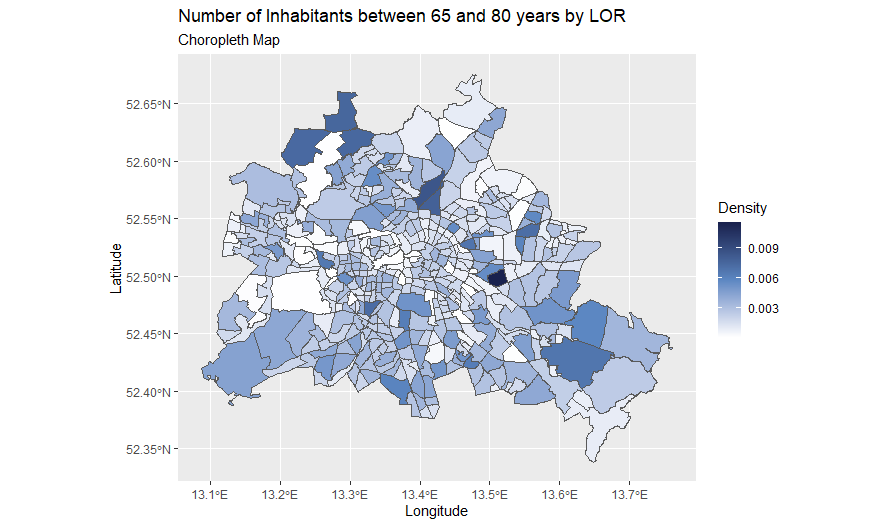
\includegraphics[scale = 0.55]{Figure/Choropleth_Part1.png}
    \caption{Choroleth map of the proportion of inhabitants between 65 and 80 years by LOR in Berlin}
    \label{fig:NoByDistric}
\end{figure}

As the discontinuities at the boundaries reflect an unrealistic scenario, the kernel heaping algorithm is applied to the data. First the data must be prepared for this application.
One of the input variables of the \texttt{dshapebivr}, which is used to evaluate the proposed approach, are the centroids of each LOR. Therefore, the \texttt{Berlin} data of type \texttt{sf} is converted to a \texttt{Large SpatialPolygonsDataFrame}. 
The \texttt{lapply} function allows in an easy way to obtain from each polygon the centroids, and the number of people between 65 and 80 years in the form of a data matrix. 
The midpoint of the  $i^{th}$ polygon out of the 447 are given at \texttt{Berlin@polygons[[i]]@Polygons[[1]]@labpt} and the total number of people in this certain age are given in \texttt{data\$E\_E65U80[i]}.
In this case, the function being used is \texttt{function(x) x@lapt}, which obtains the midpoint of each polygon. Additionally, the total number of peoples between 65 and 80 are added to the data matrix. 

\begin{example}
    # Create data frame with midpoint of areas and counts per area
    Berlin.shp <- as_Spatial(Berlin)
    dataIn <- lapply(Berlin.shp@polygons, function(x) x@labpt) %>%
      do.call(rbind, .) %>% cbind(data$E_E65U80)
    head(dataIn)
             [,1]     [,2] [,3]
    [1,] 13.34749 52.50644  562
    [2,] 13.35580 52.51386   24
    [3,] 13.35870 52.50350  639
    [4,] 13.36822 52.50211  261
    [5,] 13.36617 52.50796  120
    [6,] 13.38190 52.51102  282
\end{example}

The result of this procedure is stored in the data matrix \texttt{dataIn}. Considering the calculated table, it can be deduced that the first two columns represent the latitude and longitude of the midpoint coordinate of each polygon and the third column represents the total number of people of the observed age group in the area. 

The most important component of this code is the function \texttt{dshapebivr} of the package \hyperlink{https://cran.r-project.org/web/packages/Kernelheaping/index.html}{\pkg{Kernelheaping}}, which iteratively calculates the bivariate kernel density with respect to the people in a certain age range using the SEM algorithm. 
The function needs as an input the data frame obtained in the last step as well as the shapefile \texttt{Berlin.shp}.
In the case study, the \texttt{gridsize} for evaluating the KDE is set to 325.
Furthermore, it is important to choose an adequate number of burn-in iterations and further sample iterations for the kernel heaping function to yield accurate results. The proposed algorithm requires a few steps to converge to a realistic kernel density. 
In this case, the first 5 burn-in iterations are ignored, and the average of the last 10 iterations is calculated and returned as an estimate.
The \texttt{adaptive} parameter controls whether an adaptive smoothing factor is applied for boundary correction. 
In this case, it is set to \texttt{FALSE}, indicating that no further smoothing is utilized. 
The parameter \texttt{boundary} refers to the adjustment of the kernel density estimation near the boundaries. \cite{Jones1993} emphasizes the significance of this correction: "If a probability density function has bounded support, kernel density estimates often overspill the boundaries and are consequently especially biased at and near these edges." Therefore, correcting the density close to boundaries can reduce the induced bias. The bandwidth matrix $H$ is computed by the plug-in method proposed by \cite{Wand94}. 
\begin{example}
    # Use aggregated data to obtain KDE 
    est <- dshapebivr(data = dataIn, burnin = 5, samples = 10, 
                      adaptive = FALSE, shapefile = Berlin.shp, 
                      gridsize = 325, boundary = TRUE)
\end{example}

The result of the algorithm was stored in the data list \texttt{est}. In \texttt{est\$Mestimate} the averaged KDEs over the sampling phase is stored. The KDEs in the algorithm are calculated by the function \texttt{kde} of the package \hyperlink{https://cran.r-project.org/web/packages/ks/index.html}{\pkg{ks}}. In \texttt{est\$resultDensity} and \texttt{est\$resultX} the matrices with estimated density for each iteration respectively true latent values X of the estimated geocoordinates are stored. 
The input shapefile \texttt{Berlin.shp} and data matrix \texttt{dataIn} are also stored in \texttt{est}. The grid points needed to evaluate the KDE can be found in \texttt{est\$gridx} and \texttt{est\$gridy}. Additionally, the values for sample size,  burn-in and adaptive are stored in \texttt{est}. 

In order to plot the result, the data frame \texttt{Kdata} with all combinations of grid points with respect to their longitude and latitude coordinates as well as the corresponding density estimation obtained by the proposed algorithm is needed. The function \texttt{expand.grid} creates a data frame from all combinations of the supplied variables.
Then the normed density per grid cell is added to the data frame. 
Additionally, the function \texttt{filter} ensures that only grid points with positive densities are included in the data frame.
The data \texttt{Kdata} can now be visualized using the \hyperlink{https://cran.r-project.org/web/packages/ggplot2/index.html}{\pkg{ggplot2}} package, which provides various options for graphical representations.

\begin{example}
    # Prepare KDE as data frame for plot
    Kdata <- data.frame(expand.grid(long = est$Mestimates$eval.points[[1]],
                                    lat = est$Mestimates$eval.points[[2]]),
                        Density = est$Mestimates$estimate %>% as.vector) %>% 
      filter(Density > 0)
    Kdata$Density <- Kdata$Density*(est$gridx[2] - est$gridx[1])*
      (est$gridy[2] - est$gridy[1])
    
    # Plot KDE obtained by aggregated data 
    ggplot(Kdata) +
      geom_raster(aes(long, lat, fill = Density)) + 
      ggtitle("Density of Inhabitants between 65 and 80 Years", 
              "obtained by using Kernel Heaping Algorithm") +
      scale_fill_gradientn(colours = c("#FFFFFF", "#5c87c2", "#19224e"))+
      xlab("Longitude")+ylab("Latitude")+
      geom_sf(data = Berlin, fill = NA) + 
      coord_sf()
\end{example}

Figure \ref{fig:BivDensity} illustrates the bivariate density of elderly inhabitants by using the proposed approach. 
The impact of kernel heaping becomes evident when comparing Figure \ref{fig:BivDensity} with the conventional choropleth maps commonly used in official statistics shown in Figure \ref{fig:NoByDistric}.
Figure \ref{fig:NoByDistric} appears unrealistic compared to Figure \ref{fig:BivDensity} due to the abrupt color shifts at the boundaries of the regions. The discrete color display obscures information, i.e. regional concentrations within the districts remain hidden.

\begin{figure}[h]
    \centering
    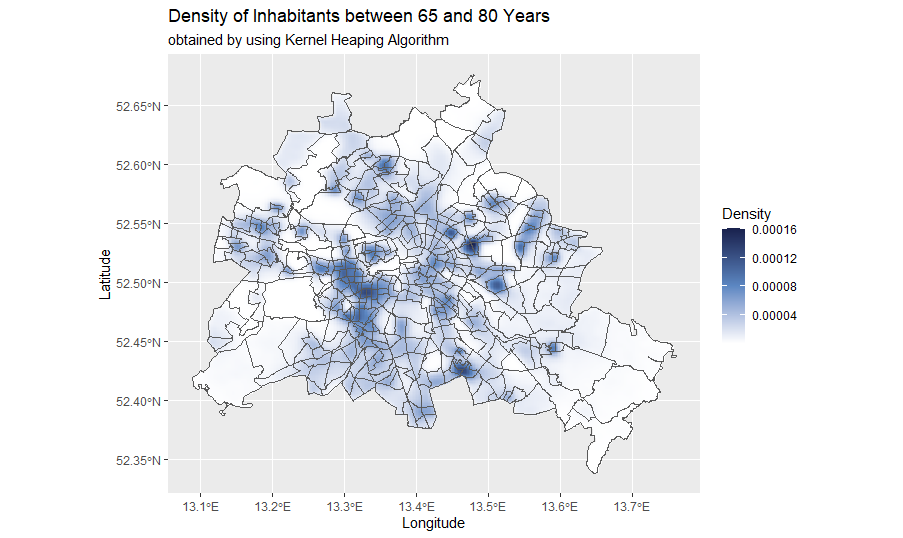
\includegraphics[scale = 0.55]{Figure/KH_Part1.png}
    \caption{Bivariate density of the number of inhabitants between 65 and 80 years in Berlin obtained by the SEM algorithm}
    \label{fig:BivDensity}
\end{figure}

\subsection{Part 2: Creating spatial maps for proportions}

This section focuses on creating maps which calculate \textbf{proportions} using data of individuals with a Turkish migration background within the population with migration background of Berlin. 

To ensure that only settled areas are considered, it is necessary to exclude unsettled regions such as parks, lakes or forests. The corresponding shape files for uninhabited areas can be downloaded from \url{http://download.geofabrik.de/europe/germany/berlin.html}. Similar to the previous section, the shape file containing the LORs of Berlin is uploaded in \pkg{R}. Additionally, land use data \texttt{BerlinN} and water areas \texttt{BerlinWater} are loaded in \pkg{R}. Land use characterizes what an area is used for, e.g., residential, commercial activities, agriculture, education, recreation, etc. and water areas refers to areas with rivers, lakes etc. The residential areas are then exempted from \texttt{BerlinN} and further divided into green areas and other areas, to distinguish between different land uses within the unsettled regions.  
\begin{example}
    # Load Berlin shape files
    Berlin <- read_sf("RBS_OD_LOR_2015_12/RBS_OD_LOR_2015_12.shp")
    Berlin <- st_transform(Berlin, CRS("+proj=longlat +datum=WGS84"))

    # Load shape files of green area, water areas and others 
    BerlinN <- read_sf("berlin-latest-free.shp/gis_osm_landuse_a_free_1.shp")
    BerlinWater <- read_sf("berlin-latest-free.shp/gis_osm_water_a_free_1.shp")
    
    BerlinN <- BerlinN[!(BerlinN$fclass == "residential"), ]
    BerlinGreen <- BerlinN[(BerlinN$fclass %in% c("forest", "grass", "nature_reserve",
                                                       "park", "cemetery","allotments",
                                                       "farm", "meadow","orchard",
                                                       "vineyard","heath")), ]
    BerlinOther <- BerlinN[!(BerlinN$fclass %in% c("forest", "grass", "nature_reserve",
                                                        "park", "cemetery","allotments",
                                                        "farm", "meadow","orchard",
                                                        "vineyard","heath")), ]
\end{example}

After reading in the shape file corresponding to the unsettled areas by using \texttt{read\_sf}, the data is again transformed into WGS84 system by \texttt{st\_transform}. Additionally, to reduce the complexity of the polygons, they are simplified by the Ramer-Douglas-Peucker algorithm using \texttt{ms\_simplify}. The algorithm decimates a curve consisting of line segments to a similar curve with fewer points. This is done for this case study due to computational efficiency. Since the data extend beyond the area of Berlin, i.e. the data reach as far as Brandenburg, the data must be restricted to Berlin using \texttt{st\_intersection}. 
The functions \texttt{dshapebivr} and \texttt{dshapebivrProp} require a single shape file as input data and therefore water, nature and other shape files are united by \texttt{bind\_rows} and transformed into a \texttt{Large SpatialPolygonsDataFrame} using \texttt{as\_Spatial}.

\begin{example}
    # Simplify the uninhabited areas for computational purpose
    BerlinGreen <- st_transform(
      rmapshaper::ms_simplify(BerlinGreen, keep = 0.001, keep_shapes=FALSE),
                               CRS("+proj=longlat +datum=WGS84"))
    BerlinOther <- st_transform(
      rmapshaper::ms_simplify(BerlinOther, keep = 0.001, keep_shapes=FALSE),
                               CRS("+proj=longlat +datum=WGS84"))
    BerlinWater <- st_transform(
      rmapshaper::ms_simplify(BerlinWater, keep = 0.001, keep_shapes=FALSE),
                               CRS("+proj=longlat +datum=WGS84"))

    BerlinOther <- st_intersection(BerlinOther, Berlin)
    BerlinGreen <- st_intersection(BerlinGreen, Berlin)
    BerlinWater <- st_intersection(BerlinWater, Berlin)

    BerlinUnInhabitated <- bind_rows(BerlinWater, BerlinGreen, BerlinOther)
    BerlinUnInhabitated <- as_Spatial(BerlinUnInhabitated)  
   
\end{example}

The differences between the simplified polygons and the original one strongly depend on the parameters. However, also small changes can achieve run time reductions. In Figure \ref{fig:water} the polygons with respect to the water areas of Berlin are plotted. It can be seen that the tuning parameter was chosen to large, hence it had a significant impact on the areas. For to enhance the readability, the code for Figure \ref{fig:water} is not provided. 

\begin{figure}[h]
    \centering
    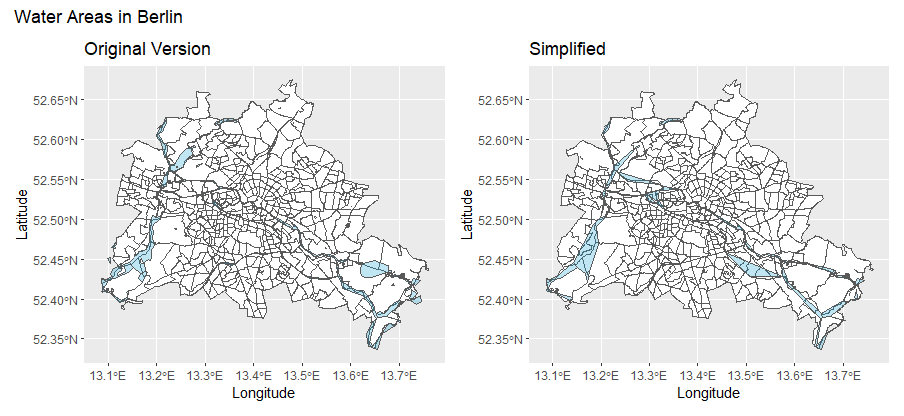
\includegraphics[scale = 0.55]{Figure/Water_Part2.png}
    \caption{Original data of the water areas in Berlin (left) based on polygons and simplified polygons using Ramer-Douglas-Peucker algorithm with a tolerance value of 0.002 (right)}
    \label{fig:water}
\end{figure}

The data for this application contains the total number of migrants in Berlin are uploaded in \pkg{R}. The CSV file can be found under \url{https://www.statistik-berlin-brandenburg.de/opendata/EWRMIGRA201512H_Matrix.csv}. At this stage, the key variable \texttt{RAUMID} is converted into a character variable. Additionally, as the length of the variable \texttt{RAUMID} is between 7 and 8, all variables are transformed to the length of 8. Therefore, the leading digits of variables of length 7 in the \texttt{RAUMID} is padded with a 0 to ensure consistent formatting. Finally, the number of migrants can be sorted in ascending order based on the \texttt{RAUMID}. 

Similar to the first part, a data matrix is determined to connect the midpoints of the polygons with the corresponding total number of Turkish migrants. Therefore, the longitude and latitude information of the midpoints are connected with the corresponding number of Turkish migrants as well as the total number of migrants. Note that in this application the \texttt{Large SpatialPolygonsDataFrame} called \texttt{Berlin.shp} is used to determine the midpoints of each LOR.


\begin{example}
    # Load data frame with migrant data
    BerlinMigration <- read.csv2("EWRMIGRA201512H_Matrix.csv")
    BerlinMigration$RAUMID <- as.character(BerlinMigration$RAUMID)
    BerlinMigration$RAUMID[nchar(BerlinMigration$RAUMID) == 7] <- 
      paste0("0", BerlinMigration$RAUMID[nchar(BerlinMigration$RAUMID) == 7])
    BerlinMigration <- BerlinMigration[order(BerlinMigration$RAUMID), ]

    # Add proportion of Turkish mirgants to shape file
    Berlin$turkDensity <- BerlinMigration$HK_Turk / BerlinMigration$MH_E
\end{example}

In Figure \ref{fig:TurkMigrantsChoropletMap} the proportion of Turkish migrants with respect to all migrants is shown as a chorophlet map. 
Note that in the KDE evaluation using SEM algorithm the unsettled areas have been excluded. However, when visualizing the proportions of migrants using choropleth maps, these areas are not excluded.
Therefore, in Figure \ref{fig:TurkMigrantsChoropletMap} the intersections between the visualized proportions of migrants and unsettled areas are displayed. This is an additional disadvantage of the common used chorpleth map. In dark green Berlin's Green areas (forests, parks, etc.), in blue Berlin's Water Areas (rivers, lakes, etc.) and in grey Berlin's other unsettled areas are visualized. 

\begin{example}
    # Plot proportions of Turkish mirgants as choropleth map 
    ggplot() +
      geom_sf(data = Berlin, mapping = aes(fill = turkDensity)) + 
      ggtitle("Proportion of Turks in Population with Migration Background", 
              subtitle = "Choropleth Map") +
      scale_fill_gradientn(colours = c("#FFFFFF", "coral1"), "Density") +
      geom_sf(fill = "grey20", alpha = .25,color = NA, 
                   data = BerlinOther) +
      geom_sf(fill = "darkolivegreen3", color = NA,
                   data = BerlinGreen, alpha = 0.25) +
      geom_sf(fill = "deepskyblue3",color = NA,
                   data = BerlinWater, alpha = 0.25) +
      xlab("Longitude")+ ylab("Latitude")+
      coord_sf()
\end{example}

\begin{figure}[h]
    \centering
    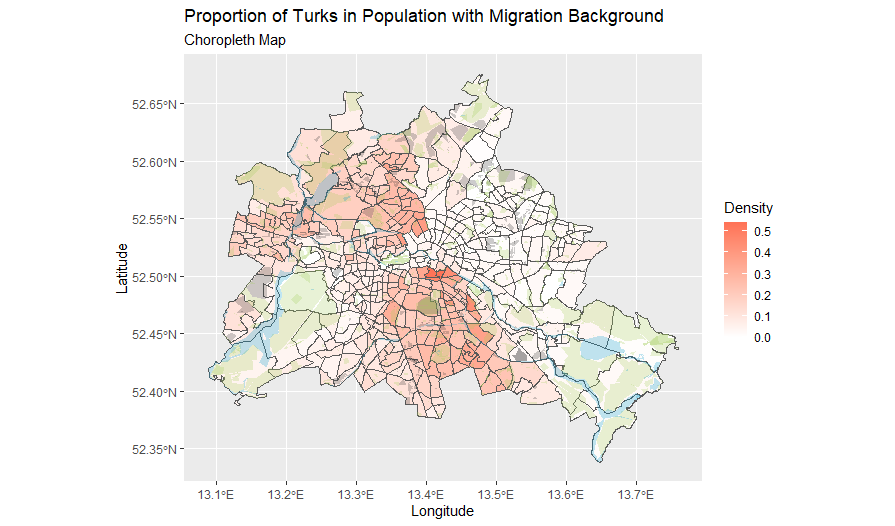
\includegraphics[scale = 0.55]{Figure/Chorophlet_Part2.png}
    \caption{Choropleth map of the proportion of Turkish people in the population with migration background per LOR}
    \label{fig:TurkMigrantsChoropletMap}
\end{figure}


\begin{example}
    # Create data frame with midpoint of areas, counts of overall population 
    # and Turkish population per area
    dataTurk <- cbind(t(sapply(1:length(Berlin.shp@polygons),
                               function(x) Berlin.shp@polygons[[x]]@labpt)),
                      BerlinMigration$HK_Turk, BerlinMigration$MH_E)
\end{example}

The function \texttt{dshapebivrProp} shares many similarities with \texttt{dshapebivr} as both are used to estimate kernel density for data classified in polygons by using SEM algorithm based on heaped data. Most of the parameters used in \texttt{dshapebivrProp} are the same as in \texttt{dshapebivr}. However, \texttt{dshapebivrProp} specifically focuses on estimating the density proportions. Additionally, in this application uninhabited areas are removed using the parameter \texttt{deleteShapes}. 

\begin{example}
    # Use aggregated data to obtain local proportions
    EstTurk <- dshapebivrProp(data = dataTurk, burnin = 5, samples = 10,
                              adaptive = FALSE, deleteShapes = BerlinUnInhabitated,
                              shapefile = Berlin.shp, gridsize = 325, boundary = TRUE,
                              numChains = 4, numThreads = 4)
\end{example}

The output \texttt{EstTurk} is similar to the output \texttt{est} of the function \texttt{dshapebivr} in Part 1. \texttt{EstTurk} consist of input information such as \texttt{shapefile, burnin, sample, deleteShape} etc. Most important is, however, \texttt{Mestimate} the corrected KDE using the proposed approach. 

For visualizing the KDE, all grid points are obtained by getting all combinations of longitude and latitude coordinates using \texttt{expand.grid}. Again, negative proportion values are filter out.
In Figure \ref{fig:turkMigrantsKDE} the KDE using the proposed approach of the proportions of Turkish migrants with respect to all migrants are visualized. As uninhabited areas are excluded from the estimation, in comparison to the choropleth map in Figure \ref{fig:TurkMigrantsChoropletMap}, no values occur in these areas as well as smooth transitions of the proportions are visible. 


\begin{example}
    # Prepare local proportions as data frame for plot
    gridBerlin <- expand.grid(long = EstTurk$Mestimates$eval.points[[1]],
                          lat = EstTurk$Mestimates$eval.points[[2]])
    KdataTurk <- data.frame(gridBerlin,                        
                            Proportion = EstTurk$proportions %>% as.vector)  %>% 
                            filter(Proportion > 0)

    # Plot local proportions obtained from aggregated data
    ggplot() +
      geom_tile(data = KdataTurk, aes(long, lat, fill = Proportion)) + 
      ggtitle("Proportion of Turks in Population with Migration Background", 
              "obtained by using Kernel Heaping Algorithm") +
      scale_fill_gradientn(colours = c("#FFFFFF", "coral1"), "n") +
      geom_sf(fill = "grey20", alpha = .25,color = NA,
              data = BerlinOther) +
      xlab("Longitude")+ ylab("Latitude")+
      geom_sf(fill = "darkolivegreen3", color = NA,
              data = BerlinGreen, alpha = .25) +
      geom_sf(fill = "deepskyblue3",color = NA,
              data = BerlinWater, alpha = .25) +
      xlab("Longitude")+ ylab("Latitude")+
      coord_sf()
\end{example}

\begin{figure}[h]
    \centering
    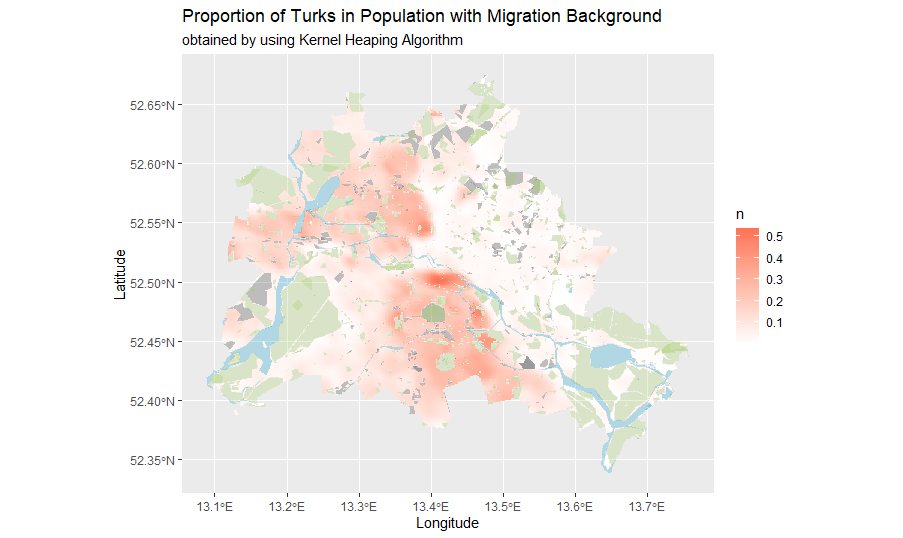
\includegraphics[scale = 0.55]{Figure/KH_Part2.png}
    \caption{Kernel Density of the Proportion of Turkish people in the population with migration background using proposed approach}
    \label{fig:turkMigrantsKDE}
\end{figure}

\subsection{Part 3: Identification of high density areas}

In the final part, the focus lies on the identification of high-density regions using the example of different migration groups in Berlin.

Similar to the previous part, the centers of the polygons are linked with the total number of Arabic, former Soviet Union, and Polish migrants. The bivariate kernel density by the proposed approach is then evaluated using \texttt{dhapebivr} with similar input parameters as in Part 1.

\begin{example}
    # Create data frame with midpoint of areas, counts of overall population 
    # and Arabic, former Soviet and Polish population per area
    dataArab <- cbind(t(sapply(1:length(Berlin.shp@polygons),
                               function(x) Berlin.shp@polygons[[x]]@labpt)),
                               BerlinMigration$HK_Arab)
    dataSU <- cbind(t(sapply(1:length(Berlin.shp@polygons),
                             function(x) Berlin.shp@polygons[[x]]@labpt)), 
                             BerlinMigration$HK_EheSU)
    dataPol <- cbind(t(sapply(1:length(Berlin.shp@polygons),
                              function(x) Berlin.shp@polygons[[x]]@labpt)), 
                              BerlinMigration$HK_Polen)

    # Use aggregated data to obtain local propotions
    EstArab <- dshapebivr(data = dataArab, burnin = 5, samples = 10, adaptive = FALSE,
                          shapefile = Berlin.shp, gridsize = 325, boundary = TRUE)
    EstSU <- dshapebivr(data = dataSU, burnin = 5, samples = 10, adaptive = FALSE,
                        shapefile = Berlin.shp, gridsize = 325, boundary = TRUE)
    EstPol <- dshapebivr(data = dataPol, burnin = 5, samples = 10, adaptive = FALSE,
                         shapefile = Berlin.shp, gridsize = 325, boundary = TRUE)
\end{example}

To identify "hot spots" or regions with significantly higher density than others, a predetermined quantile needs to be established. In this case, we set the \texttt{visquantile} to 0.95. This means that in 95 percent of the grid points the estimate of the percentage is lower than the given value. 

The data is prepared in the same manner as in the previous two parts. 

\begin{example}
    # prepare local proportions as data frame for plot
    # Plot only high density regions
    Visquantile <- 0.95
    KdataArab <- 
        data.frame(gridBerlin, Density = EstArab$Mestimates$estimate %>% as.vector) %>% 
            filter(Density > 0) %>% 
            filter(Density > quantile(Density, Visquantile)) %>% 
            mutate(Density = "Arabian countries")
    KdataSU <- 
        data.frame(gridBerlin, Density = EstSU$Mestimates$estimate %>% as.vector) %>%
            filter(Density > 0) %>% 
            filter(Density > quantile(Density, Visquantile)) %>%
            mutate(Density = "Former Soviet Union")
    KdataPol <- 
        data.frame(gridBerlin, Density = EstPol$Mestimates$estimate %>% as.vector) %>%  
            filter(Density > 0) %>% 
            filter(Density > quantile(Density, Visquantile)) %>%
            mutate(Density = "Poland")
    
    # Plot local proportions by aggregated data
    ggplot() +
      geom_sf(data = Berlin) +
      geom_tile(aes(long, lat, fill = Density), data = KdataArab, alpha = 0.6) + 
      geom_tile(aes(long, lat, fill = Density), data = KdataSU, alpha = 0.6) + 
      geom_tile(aes(long, lat, fill = Density), data = KdataPol, alpha = 0.6) +
      ggtitle("Hotspots of Inhabitants with different Migration Background", 
              "obtained by using Kernel Heaping Algorithm") +
      geom_sf(fill = "grey20", alpha = .25,color = NA,
              data = BerlinOther) +
      xlab("Longitude")+ ylab("Latitude")+
      geom_sf(fill = "darkolivegreen3", color = NA,
              data = BerlinGreen, alpha = .25) +
      geom_sf(fill = "deepskyblue3",color = NA,
              data = BerlinWater, alpha = .25) +
      xlab("Longitude")+ ylab("Latitude")+
    coord_sf()
\end{example}
The result is a hot spot map displaying the density of former Soviet Union in green, Arab in red, and Polish migrants in blue visualized in Figure \ref{fig:DifferentMigrationHotspots}.
By employing standard bivariate kernel density estimation, proportions estimation and hotspot identification techniques, it is possible to address the limitations of choropleth maps. The new resulting maps exhibit enhanced visual representation due to the incorporation of kernel heaping. This approach effectively highlights regional concentrations within the life-oriented regions (LORs) and hotspots can be identified. 

\begin{figure}[h]
    \centering
    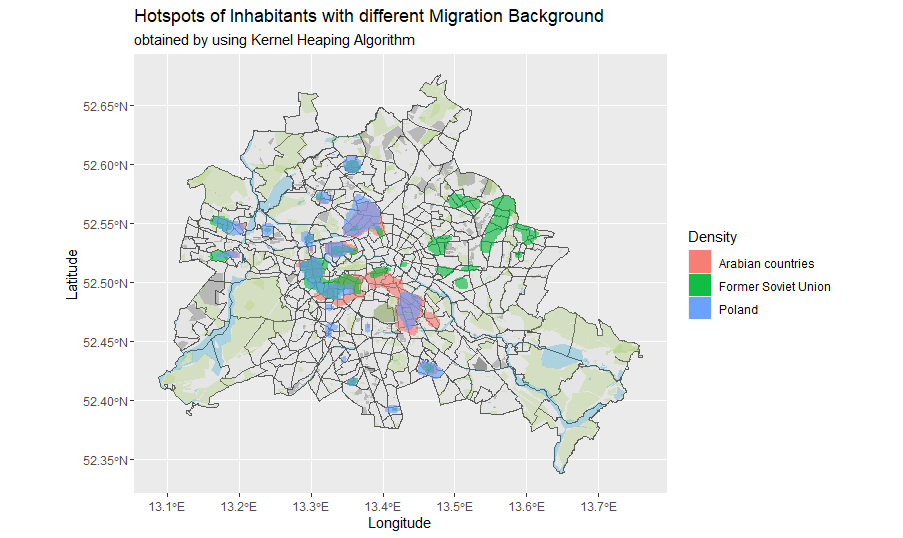
\includegraphics[scale = 0.55]{Figure/KH_Part3.png}
    \caption{Hot spots of migrants from the former Soviet Union as well as Arab, and Polish migrants constructed from the Kernel density estimates.}
    \label{fig:DifferentMigrationHotspots}
\end{figure}

\section{Robustness analysis based on a simulation study}

In order to validate the method based on different data structures, sample data points in the form of coordinates have been randomly generated with various spreads, i.e. sample data were generated from a mixture of 111 normal distributions with different standard deviations. 
For each of the 111 midpoints with varying the standard deviation, 800 coordinates were generated. The standard deviation varies from $3\cdot 10^{-4.8} \cdot I_2$, for highly agglomerated data, 
$3\cdot 10^{-4.55} \cdot I_2$, for large agglomeration clusters, to $3\cdot 10^{-3} \cdot I_2 $, for nearly uniformly distributed data. 
Additionally, a combination of these three standard deviations each associated with 37 midpoints has been used for data generation and named $C_{NMD}$. 
Since green areas, water areas and uninhabited areas in Berlin are known, those points that were randomly placed in one of these areas or fell outside of Berlin were excluded. Each setting has been randomly simulated 500 times. 
Figure \ref{fig:setting_variation} shows the data variations and is intended to represent the highly agglomerated data ($3\cdot 10^{-4.8} \cdot I_2$), less agglomerated data ($3\cdot 10^{-4.55} \cdot I_2$), nearly equally distributed data ($3\cdot 10^{-3} \cdot I_2$) and data resulting from the combination of 3 different standard deviations ($C_{NMD}$).  


\begin{figure}[ht]
    \centering
    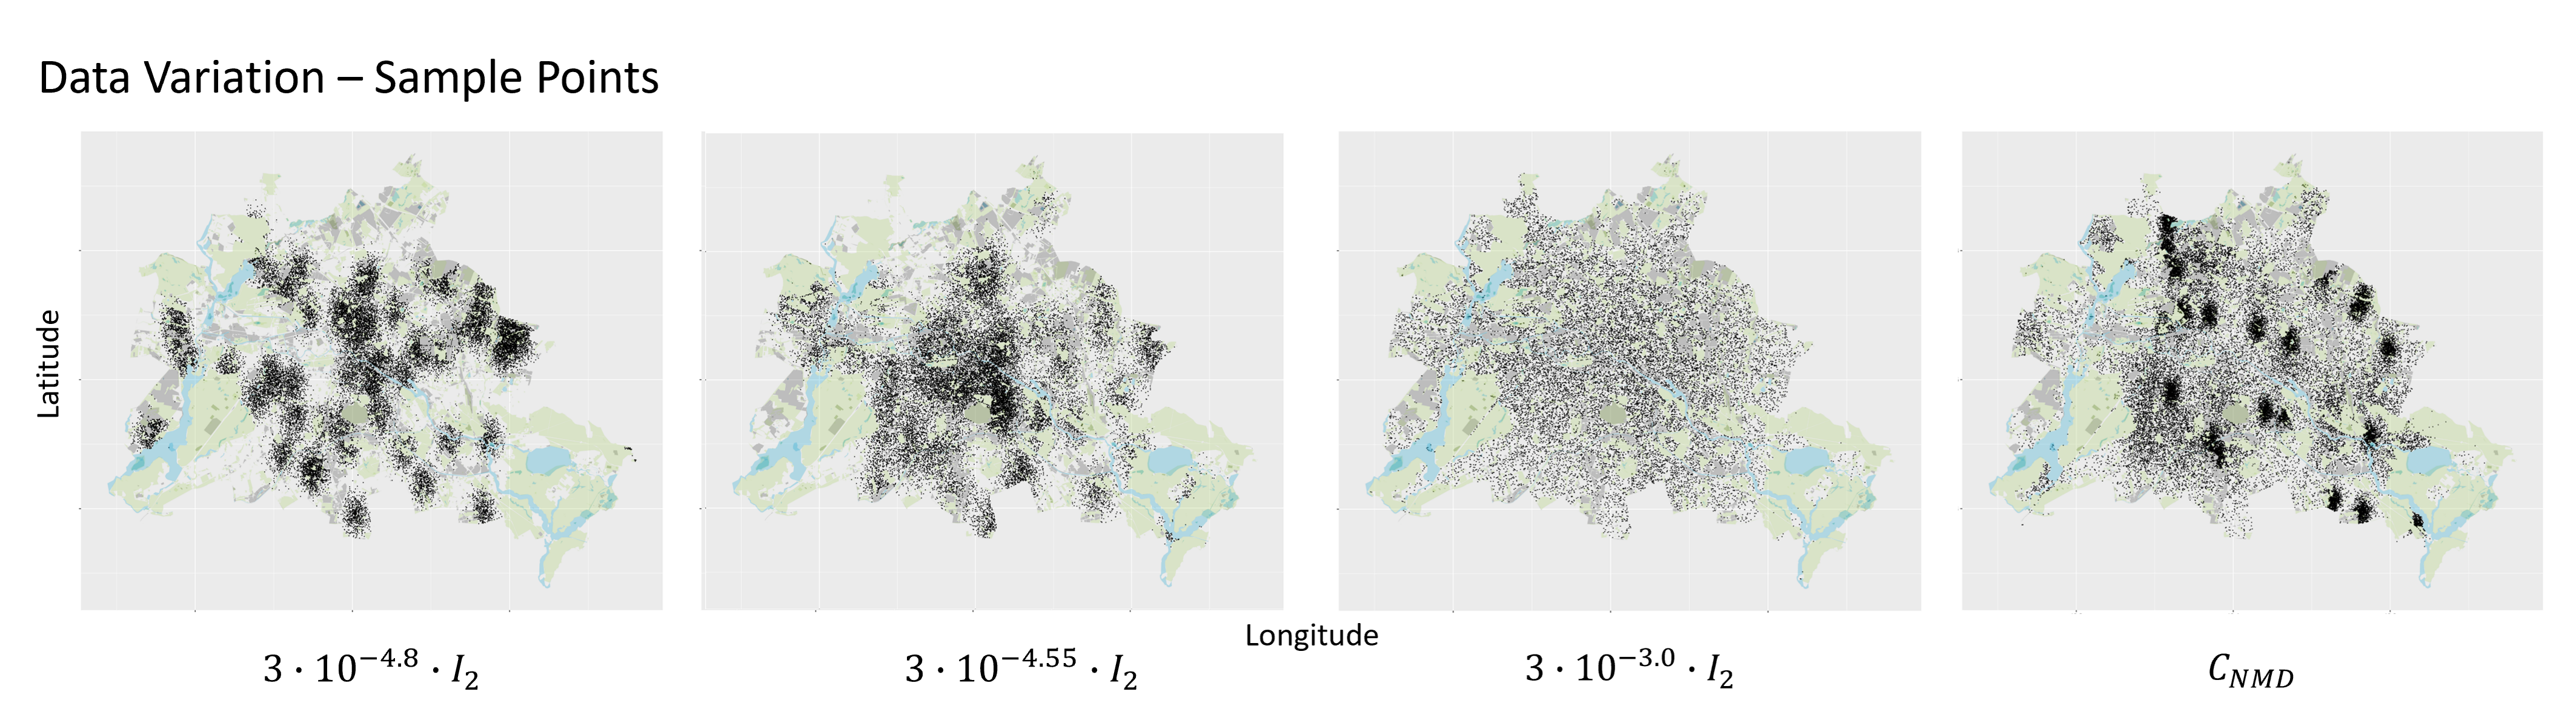
\includegraphics[scale = 0.42]{Figure/Setting_Variation2.png}
    \caption{Different data generation processes by using Gaussian Mixture distribution with various variances}
    \label{fig:setting_variation}
\end{figure}

Based on these data structures, the randomly drawn sample points have been aggregated to a wide range of area systems, i.e. from districts with 12 areas,
and Prognosis areas with 60 areas to Zip codes with 193 areas and Lifeworld-oriented spaces with 442 areas.
Based on aggregated data, the kernel heaping method aiming for a smooth representation is applied. 
For the comparison of two densities over the considered domain, the Root Mean Integrated Squared Error ($RMISE$) is used, which is defined for the true density $f$ and the estimated density $\hat{f}_H$ as  
$$ RMISE(f, \hat{f}_H) = \frac{1}{G} \sum_{g = 1}^G (f(x_g) - \hat{f}_H(x_g))^2 \Delta_\mathcal{G}. $$
Figure \ref{fig:NormedRMISE} shows the information loss for different variants of the data structures on the horizontal axis, as well as aggregation error and simulated smoothing error by kernel heaping as separated plots.
The information loss is determined by normalizing the considered error by the sampling error, which occurs through drawing samples from the known mixture of normal distributions. The aggregation of the sampling data points on area systems with fewer areas highly increases the aggregation error. Additionally, the data structure is influential. The kernel heaping algorithm uses the aggregated information to generate a smooth density through the SEM algorithm. This smooth density drastically reduces the loss of information which is enhanced by the smoothing effect of the algorithm. Nevertheless, for highly agglomerated data the effect is less because highly agglomerated data clusters cannot be reconstructed, i.e. when multiple clusters have been aggregated into one area. 
The simulation study shows that an information loss between 25\% and 50\% can be improved with respect to $RMISE$, depending on the underlying data structure. 

\begin{figure}[ht]
    \centering
    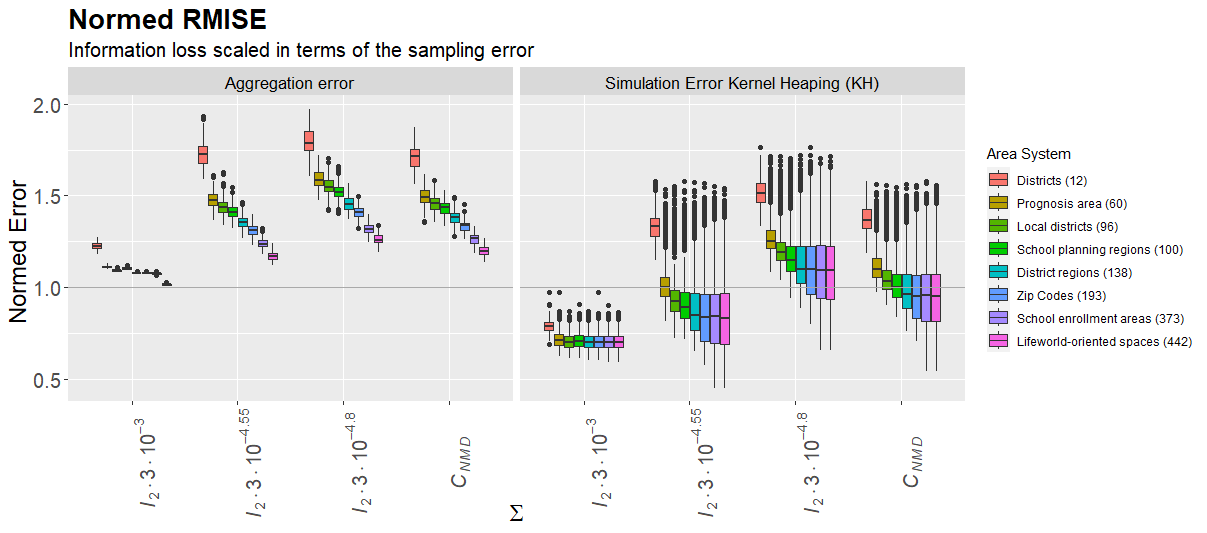
\includegraphics[width = \textwidth]{Figure/NormedRMISE.png}
    \caption{Information Loss by Normed Root Mean Integrated Squared Error with respect to the Sampling Error for Aggregation processes as well as Kernel Heaping compared to true density for different area systems and data gerneration processes.}
    \label{fig:NormedRMISE}
\end{figure}

The computation time depends strongly on the grid used to evaluate the kernel density. 
The finer the grid, the longer the computation time.
To generate a $100 \times 100$ meter grid over Berlin, which has an extension of 45 km in north-south direction and 38 km in east-west direction, the area has to be divided into 450 and 380 grid cells per direction, respectively.  
As the number of grid cells decreases, the computation time decreases. 
In general, as the number of areas on which the aggregation is based increases, the computation time increases, as seen in the table \ref{tab:my_label2}. 
The data structure on which the aggregation is based plays a minor role and causes the results to vary by a few seconds. Note that a burn-in phase of 5 iterations and a sampling phase of 10 iterations are used. The computations are based on a 12th Gen Intel(R) Core(TM) i5-12500, 3000 MHz, 6 cores processor. 

\begin{longtable}{|l || l| l |l | l| l | l | l| l | }
  % \centering
    %\begin{tabular}{ }
    \hline
    Number of Areas & 12 & 60 & 96 & 100& 138 & 193 & 373 & 442 \\
    \hline 
    % Mean Computation Time  & & & & & & & & \\
    100m $\times$ 100m &  270.99 & 282.96 & 304.64 & 277.95 & 287.09& 316.71 & 309.90 & 301.75 \\ 
    200m $\times$ 200m &  62.02 &  62.87 &  69.86 &  64.09&  64.41&  70.34&  70.33&  67.95 \\
    500m $\times$ 500m & 14.33&   13.98& 14.78& 14.45& 15.01&  14.46&
   14.73& 15.11  \\
    \hline
    %\end{tabular}
    \caption{Overview of the mean computation time (in seconds) for different area systems and grid sizes}\label{tab:my_label2}
\end{longtable}

\subsection{Kernel Heaping under different Bandwidth selectors}

An automatic bandwidth selection via the plug-in bandwidth by \cite{Wand94} is implemented in the \hyperlink{https://cran.r-project.org/web/packages/Kernelheaping/index.html}{\pkg{Kernelheaping}} package. 
The calculation of the KDE in each iteration step is based on the \texttt{kde()} function of the \hyperlink{https://cran.r-project.org/web/packages/ks/index.html}{\pkg{ks}} package, which offers other automatic bandwidth calculation methods besides the plug-in bandwidth. 
In addition to the plug-in bandwidth, the biased cross-validation (BCV) bandwidth matrix selector by \cite{Sain1994}, the smoothed cross-validation (SCV) bandwidth selector by \cite{Duong2005} and the least-squares cross-validation (LSCV) bandwidth selector by \cite{Bowman} are evaluated.
Instead of minimizing $AMISE(H)$ by an plug-in approach, cross-validation based approaches attempt to minimize the $MISE$ by using data for KDE computation and evaluation of its performance. To avoid dependencies the data for computation is not used for evaluation. The least-squares cross validation selector uses a leave-one-out approach and numerical minimization. The biased cross validation combines the plug-in approach with the idea of cross validation. By considering to minimize the $AMISE(H)$ an estimation of $\phi_4$ is modified by an leave-out-diagonals approach. For details see \cite{Sain1994}. Note that there are two BCV estimates, where the first is used in this simulation.  
The smoothed cross-validation can be viewed as a combination of the LSCV and BCV
\cite{Duong2005}. \\
\begin{figure}[ht]
    \centering
    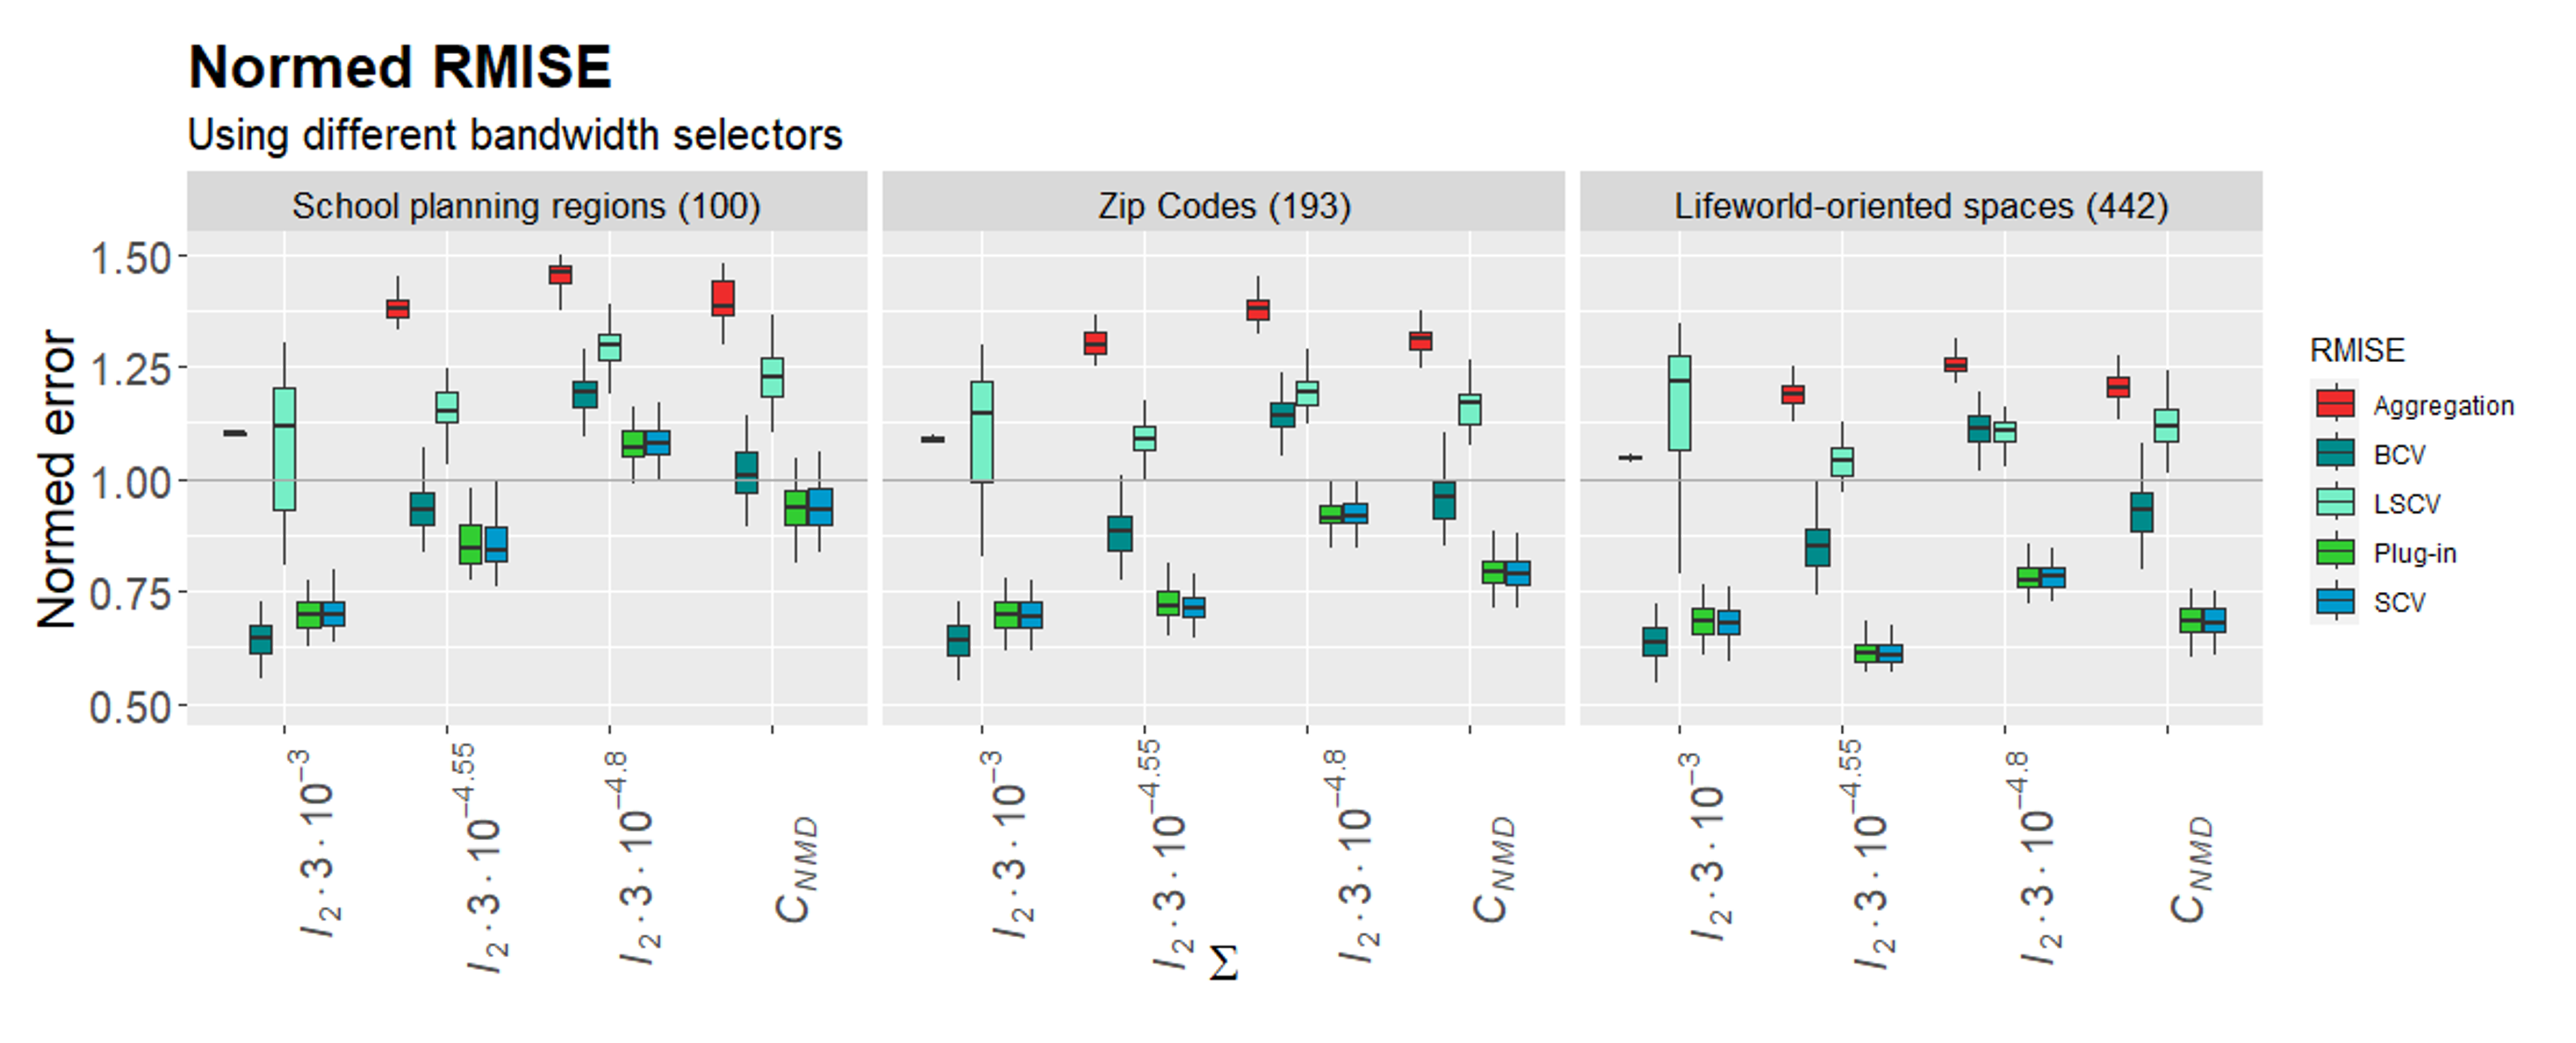
\includegraphics[width = \textwidth]{Figure/NormedRMISEBandwidth.png}
    \caption{Information Loss by Normed Root Mean Integrated Squared Error for Aggregation process and Kernel Heaping using different bandwidth selectors under selected area systems and different data generation processes }
    \label{fig:NormedRMISEBandwidth}
\end{figure}

In Figure \ref{fig:NormedRMISEBandwidth} the information loss based on the normed $RMISE$ for different automatic bandwidth selectors is compared with the information loss of the aggregation process. 
As before, sample data from a Gaussian mixture distribution have been aggregated to three selected area systems. Based on the aggregated data the kernel heaping algorithm is applied with different automatic bandwidth selectors on a $500 \times 500$ meter grid. The plug-in bandwidth selector which used in the \hyperlink{https://cran.r-project.org/web/packages/Kernelheaping/index.html}{\pkg{Kernelheaping}} is compared to the BCV, LSCV and SCV. 
Expect from nearly equally distributed data combined with the LSCV, the kernel heaping algorithm could reduce the information loss. The LSCV bandwidth selector performed worse followed by the BCV. The plug-in bandwidth selector and the SCV bandwidth selector perform similarly well in the context of the global error measure. Nevertheless, the mean computation time of the SCV is approximately 3.6 times higher compared to the plug-in bandwidth selector. 
For school planning regions, for example, the mean computation time of the $C_{NMD}$ setting is 
15.75 seconds for the plug-in selector compared to 56.52 seconds for the SCV selector. Note that the computation time for LSCV is 112.40 seconds and for BCV 332.53 seconds. 
Hence, compared to these automatic bandwidth selectors the plug-in bandwidth is very efficient. The computations are based on a 12th Gen Intel(R) Core(TM) i5-12500, 3000 MHz, 6 cores processor. 


\section{Summary}

The \hyperlink{https://cran.r-project.org/web/packages/Kernelheaping/index.html}{\pkg{Kernelheaping}} package is a useful tool for representing georeferenced data, which are given only as aggregates, by realistic kernel density estimates. Among the two dimensional cases shown, the implementation in \pkg{R} can be used for one dimensional rounding effects as well as three dimensional data established in the function \texttt{dshape3dprop()}. 
The focus in the case studies lied in two dimensional aggregations of population data, and in particular in the handling on shape files, etc., which are essential for georeferenced data. The function \texttt{toOtherShape} also handles the support problem, i.e. the change between non-hierarchical area systems. Since the basic idea behind the algorithm is the aggregation of populations, and the drawing of pseudo-samples reflects the drawing of a simulated population, the algorithm can only be meaningfully applied to integer non-negative values. 
In addition to the use of exemplary data of the population between 65 and 80 and people with a migration background, a simulation was conducted. It was demonstrated that the performance of the algorithm depends on both the underlying data structure and the size of the aggregation areas. Furthermore, the efficient use of the plug-in bandwidth was shown in comparison to CV-based methods.



\section{Acknowledgement}
Parts of this work was supported by the collaborative project \hyperlink{https://www.destatis.de/DE/Ueber-uns/AnigeD/_inhalt.html}{\textit{AnigeD}} under funding reference number \textit{16KISA097}. 



\bibliography{KH.bib}

\address{%
Lorena Gril\\
Freie Universität Berlin, FB Wirtschaftswissenschaft\\%
Garystr. 21, D-14195 Berlin\\ Germany\\ \url{lorena.gril@fu-berlin.de}\\
%
%
%
%
}

\address{%
Laura Steinkemper\\
Freie Universität Berlin, FB Wirtschaftswissenschaft\\%
Garystr. 21, D-14195 Berlin\\ Germany\\ \url{steinkel98@zedat.fu-berlin.de}\\
%
%
%
%
}

\address{%
Marcus Groß\\
INWT Statistics GmbH\\%
Hauptstr.8, D-10827 Berlin\\ Germany\\ \url{Marcus.Gross@inwt-statistics.de}\\
%
%
%
%
}

\address{%
Ulrich Rendtel\\
Freie Universität Berlin, FB Wirtschaftswissenschaft\\%
Garystr. 21, D-14195 Berlin\\ Germany\\ \url{Ulrich.Rendtel@fu-berlin.de}\\
%
%
%
%
}
